%!TEX program = xelatex

\documentclass[11pt,titlepage]{report}
%!TEX root = main.tex

\usepackage[T1]{fontenc}
\usepackage{lmodern}
\usepackage[svgnames]{xcolor}
\usepackage{fontspec} % XeLaTeX required!
\usepackage{graphicx}
\usepackage{circuitikz}
\usepackage{tikz}
\usepackage{pifont}
\usepackage[some]{background}
\usepackage{xltxtra} 
\usepackage{setspace}
\usepackage[absolute]{textpos}
\usepackage[latin1]{inputenc}
\usepackage[english]{babel}
\usepackage{graphicx}
\usepackage{wrapfig}
\usepackage{fullpage}
\usepackage[margin=1in]{geometry}
\usepackage{float}
\usepackage{url}
\usepackage{multicol}
\usepackage{hyperref}
\usepackage{titlepic}
\usepackage{standalone}
\usepackage{siunitx}
\usepackage{booktabs}
\usepackage{amsmath}
\usepackage{unicode-math}
\usepackage{verbatim}
\usepackage{enumitem}
\usepackage{listings}
\usepackage{multirow}
\usepackage{pgfplots}
\pgfplotsset{compat=1.8}
\usepackage{caption} 
\usepackage[parfill]{parskip}
\usepackage{import}
\usepackage[backend=bibtexu,texencoding=utf8,bibencoding=utf8,style=ieee,sortlocale=en_GB,language=auto]{biblatex}
\usepackage[strict,autostyle]{csquotes}
\usepackage[final]{pdfpages}
\usepackage{subcaption}
\usepackage{ifplatform}
%\captionsetup[table]{skip=10pt}


% Fix for includepdf bug in Mac OS X
\newcommand{\insertpdfpath}[1]{
	\ifwindows
	\newcommand{\insertpdf}[2]{\includepdf[pages=##1]{##2}}
	\else
	\newcommand{\insertpdf}[2]{\includepdf[pages=##1]{#1/##2}}
	\fi
}

%set fonts
\setmainfont[Ligatures=TeX]{Myriad Pro}
\setmathfont{Asana Math}
\setmonofont{Lucida Console}

\usepackage{titlesec, color}
\renewcommand{\familydefault}{\sfdefault} %set font family
\renewcommand{\arraystretch}{1.2} %set table vertical spacing
\setlength\parindent{0pt} %no paragraph indent
\hypersetup{ %setup hyperlinks
    colorlinks,
    citecolor=black,
    filecolor=black,
    linkcolor=black,
    urlcolor=black
}

%redesign chapter headings
\definecolor{gray75}{gray}{0.75}
\newcommand{\chapternumber}{\thechapter}
\newcommand{\hsp}{\hspace{20pt}}
\titleformat{\chapter}[hang]{\Huge\bfseries}{\chapternumber\hsp\textcolor{gray75}{|}\hsp}{0pt}{\Huge\bfseries}

%Redefine appendix headers
\renewcommand{\appendixname}{Appendix}
\renewcommand{\appendixtocname}{Appendices}
\renewcommand{\appendixpagename}{Appendices}

%For code listings
\definecolor{black}{rgb}{0,0,0}
\definecolor{browntags}{rgb}{0.65,0.1,0.1}
\definecolor{bluestrings}{rgb}{0,0,1}
\definecolor{graycomments}{rgb}{0.4,0.4,0.4}
\definecolor{redkeywords}{rgb}{1,0,0}
\definecolor{bluekeywords}{rgb}{0.13,0.13,0.8}
\definecolor{greencomments}{rgb}{0,0.5,0}
\definecolor{redstrings}{rgb}{0.9,0,0}
\definecolor{purpleidentifiers}{rgb}{0.01,0,0.01}


\lstdefinestyle{csharp}{
language=[Sharp]C,
showspaces=false,
showtabs=false,
breaklines=true,
showstringspaces=false,
breakatwhitespace=true,
escapeinside={(*@}{@*)},
columns=fullflexible,
commentstyle=\color{greencomments},
keywordstyle=\color{bluekeywords}\bfseries,
stringstyle=\color{redstrings},
identifierstyle=\color{purpleidentifiers},
basicstyle=\ttfamily\small}

\lstdefinestyle{c}{
language=C,
showspaces=false,
showtabs=false,
breaklines=true,
showstringspaces=false,
breakatwhitespace=true,
escapeinside={(*@}{@*)},
columns=fullflexible,
commentstyle=\color{greencomments},
keywordstyle=\color{bluekeywords}\bfseries,
stringstyle=\color{redstrings},
identifierstyle=\color{purpleidentifiers},
}

\lstdefinestyle{matlab}{
language=Matlab,
showspaces=false,
showtabs=false,
breaklines=true,
showstringspaces=false,
breakatwhitespace=true,
escapeinside={(*@}{@*)},
columns=fullflexible,
commentstyle=\color{greencomments},
keywordstyle=\color{bluekeywords}\bfseries,
stringstyle=\color{redstrings},
identifierstyle=\color{purpleidentifiers}
}

\lstdefinestyle{vhdl}{
language=VHDL,
showspaces=false,
showtabs=false,
breaklines=true,
showstringspaces=false,
breakatwhitespace=true,
escapeinside={(*@}{@*)},
columns=fullflexible,
commentstyle=\color{greencomments},
keywordstyle=\color{bluekeywords}\bfseries,
stringstyle=\color{redstrings},
identifierstyle=\color{purpleidentifiers}
}

\lstdefinestyle{xaml}{
language=XML,
showspaces=false,
showtabs=false,
breaklines=true,
showstringspaces=false,
breakatwhitespace=true,
escapeinside={(*@}{@*)},
columns=fullflexible,
commentstyle=\color{greencomments},
keywordstyle=\color{redkeywords},
stringstyle=\color{bluestrings},
tagstyle=\color{browntags},
morestring=[b]",
  morecomment=[s]{<?}{?>},
  morekeywords={xmlns,version,typex:AsyncRecords,x:Arguments,x:Boolean,x:Byte,x:Char,x:Class,x:ClassAttributes,x:ClassModifier,x:Code,x:ConnectionId,x:Decimal,x:Double,x:FactoryMethod,x:FieldModifier,x:Int16,x:Int32,x:Int64,x:Key,x:Members,x:Name,x:Object,x:Property,x:Shared,x:Single,x:String,x:Subclass,x:SynchronousMode,x:TimeSpan,x:TypeArguments,x:Uid,x:Uri,x:XData,Grid.Column,Grid.ColumnSpan,Click,ClipToBounds,Content,DropDownOpened,FontSize,Foreground,Header,Height,HorizontalAlignment,HorizontalContentAlignment,IsCancel,IsDefault,IsEnabled,IsSelected,Margin,MinHeight,MinWidth,Padding,SnapsToDevicePixels,Target,TextWrapping,Title,VerticalAlignment,VerticalContentAlignment,Width,WindowStartupLocation,Binding,Mode,OneWay,xmlns:x}
}

\lstdefinestyle{matlab}{
language=Matlab,
showspaces=false,
showtabs=false,
breaklines=true,
showstringspaces=false,
breakatwhitespace=true,
escapeinside={(*@}{@*)},
columns=fullflexible,
commentstyle=\color{greencomments},
keywordstyle=\color{bluekeywords}\bfseries,
stringstyle=\color{purpleidentifiers},
identifierstyle=\color{purpleidentifiers}
}

%defaults
\lstset{
basicstyle=\ttfamily\small,
extendedchars=false,
numbers=left,
numberstyle=\ttfamily\tiny,
stepnumber=1,
tabsize=4,
numbersep=5pt
}
\addbibresource{../../library/bibliography.bib}

\begin{document}

\chapter{Assignment 1: System identification}
\section{Excitation signal generation}
For identifying the parameters of the previously obtained second order model, we had to apply some form of excitation signal to KITT for him to drive, so we could measure his output. We chose to make KITT drive back and forth in a line perpendicular to a solid reference point, in our case a wall. The corresponding excitation signal was dynamically generated, depending on KITT's distance to that wall. An event based scheme of the signal generation logic is shown in Figure~\ref{fig:ass1-chain}.

\usetikzlibrary{shapes,arrows}
\tikzstyle{block} = [
	rectangle,
	draw,
	fill=blue!20, 
    text width=7em, 
    text centered,
    rounded corners,
    minimum height=4em
]
\tikzstyle{every edge} = [
	draw,
	>=triangle 90
]

\begin{figure}[H]
	\centering
	\begin{tikzpicture}[node distance = 5cm, auto]
		% Nodes
		\node [block] (initial) {Initial position};
		\node [block, right= 4cm of initial] (mindist) {Minimum distance to wall reached};
		\node [block, above= 2cm of mindist] (maxdist) {Maximum distance to wall reached};
		% Edges
		\path (initial) edge [->] node {KITT drives forward} (mindist);
		\path (mindist.100) edge [->] node {KITT drives backward} (maxdist.-100);
		\path (maxdist.-80) edge [->] node {KITT drives forward} (mindist.80);
	\end{tikzpicture}
	\caption{Event-based scheme of excitation signal generation}
	\label{fig:ass1-chain}
\end{figure}

After implementing such behaviour in MATLAB, we obtained signals during our two measurements, as shown in Figure~\ref{fig:ass1-excitation}.

\begin{figure}[H]
	\begin{subfigure}{.5\textwidth}
		\begin{center}
			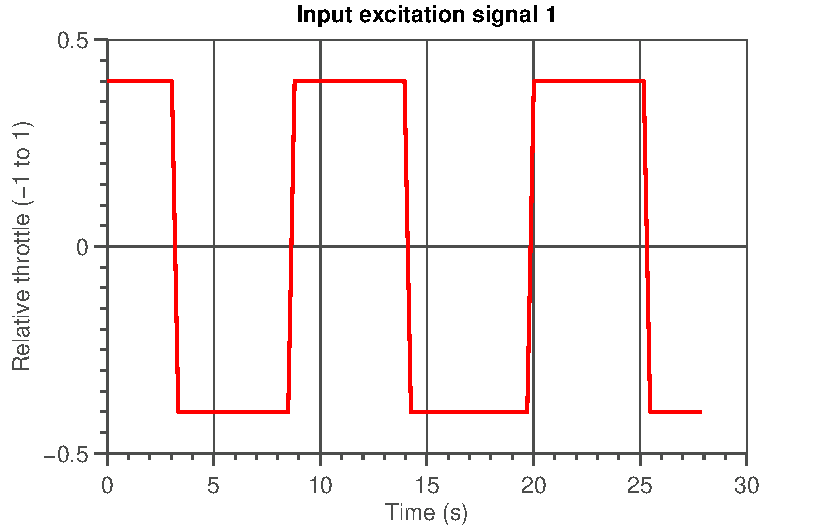
\includegraphics[width=\linewidth]{resource/drive-excitation1.pdf}
		\end{center}
	\end{subfigure}
	\begin{subfigure}{.5\textwidth}
		\begin{center}
			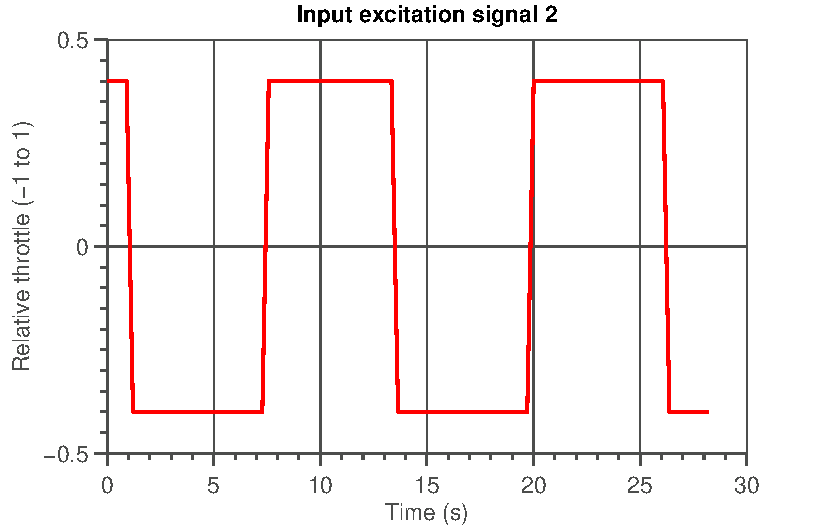
\includegraphics[width=\linewidth]{resource/drive-excitation2.pdf}
		\end{center}
	\end{subfigure}
	\caption{The drive excitation signals in our two measurements}
	\label{fig:ass1-excitation}
\end{figure}

\section{The experiment}
The output of KITT's left ultrasound sensor (being more accurate than the right one) was used for determining KITT's distance to the wall, and thus the output of the desired state space model. However, using the sensor's `raw' output data was not an option, since it would sometimes spike to zero or another random value. To overcome this, a finite impulse response (FIR) filter was implemented in the data acquisition MATLAB-script. This filter uses the last three determined values to compute an expected value for the next measurement. If this next measurement deviates too much from the expected value, the measured value is replaced with the expected value. The FIR-filter thus acts as a low-pass filter, blocking high frequency noise (sensor spikes) and passing through the actual signal.
The filtered results are shown in Figure~\ref{fig:ass1-output}.

\begin{figure}[H]
	\begin{subfigure}{.5\textwidth}
		\begin{center}
			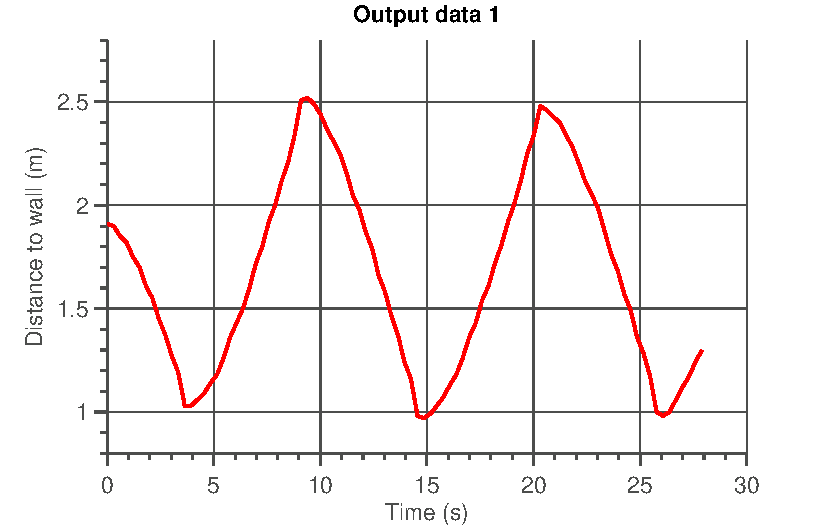
\includegraphics[width=\linewidth]{resource/distances1.pdf}
		\end{center}
	\end{subfigure}
	\begin{subfigure}{.5\textwidth}
		\begin{center}
			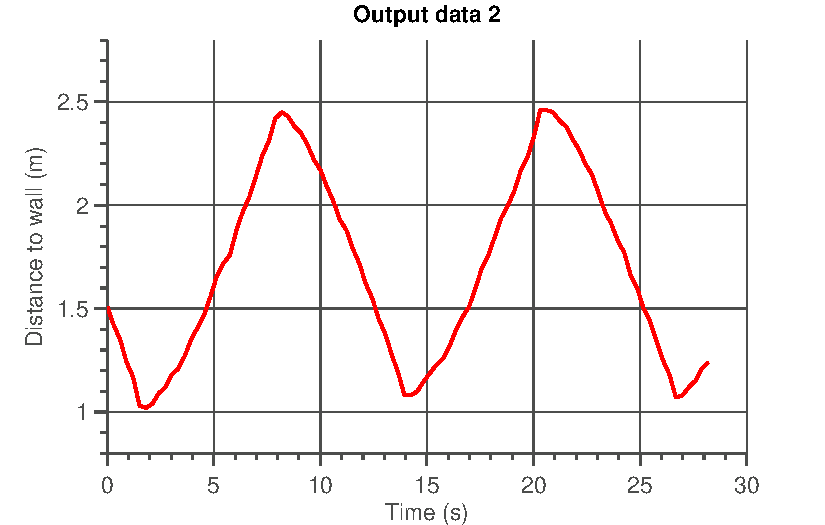
\includegraphics[width=\linewidth]{resource/distances2.pdf}
		\end{center}
	\end{subfigure}
	\caption{The measured output in our two measurements}
	\label{fig:ass1-output}
\end{figure}

These graphs resemble the behaviour we expected KITT to exhibit: driving back and forth with a relatively constant velocity.

\section{Obtaining the model}
Using MATLAB's system identification toolbox, we obtained a state space model of the ``observability canonical'' form, since this resembles the form of previously derived vehicle model best. The fitting results are shown in Figure~\ref{fig:ass1-fit}. The model was obtained using output dataset \num{1}, and validated using output dataset \num{2}.

\begin{figure}[H]
	\begin{subfigure}{.5\textwidth}
		\begin{center}
			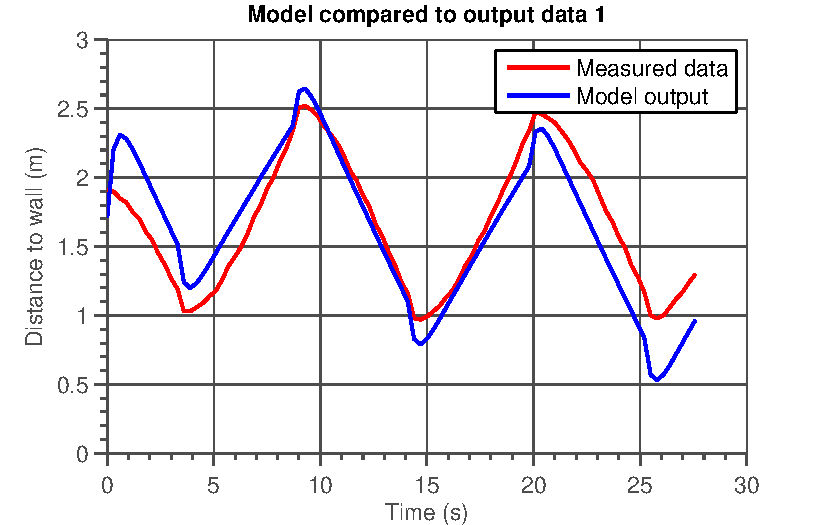
\includegraphics[width=\linewidth]{resource/model-fit1.pdf}
		\end{center}
	\end{subfigure}
	\begin{subfigure}{.5\textwidth}
		\begin{center}
			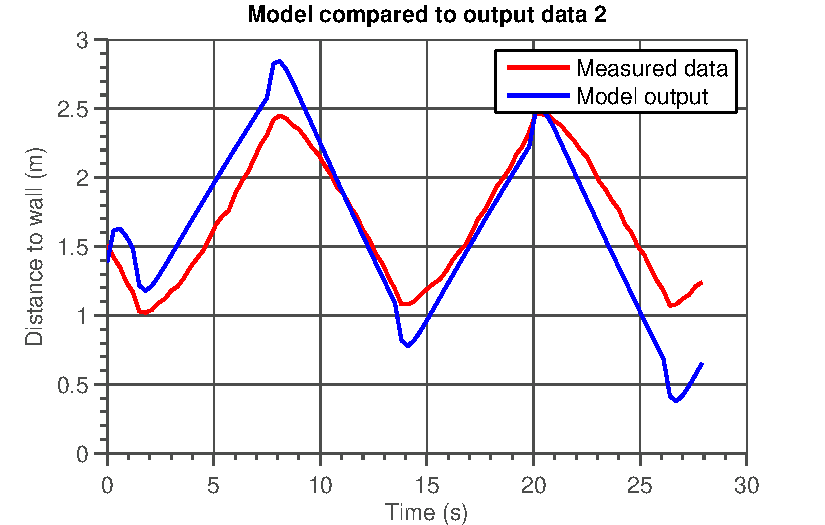
\includegraphics[width=\linewidth]{resource/model-fit2.pdf}
		\end{center}
	\end{subfigure}
	\caption{The estimated model compared to actual measured data}
	\label{fig:ass1-fit}
\end{figure}

We see that the model approaches reality pretty well, considering it being only of the second order. Being satisfied with these results, we obtained the following matrices:

\begin{equation}
	\mathbf{A} =
		\begin{bmatrix}
			0 & 1 \\
			-0.0723 & -3.4955 \\
		\end{bmatrix}
	\quad
	\mathbf{B} = 
		\begin{bmatrix}
			1.6339 \\
			-8.2873 \\
		\end{bmatrix}
		\quad
	\mathbf{C} = 
		\begin{bmatrix}
			1 \\
			0 \\
		\end{bmatrix}
	.
\end{equation}

It is worth noticing that both $a_{21}$ and $b_{1}$ are not equal to zero in this model, while they were in the previously derived one. For $a_{21}$, this implies acceleration is somehow influenced by the current position of KITT , which would be rather strange. These anomalies can be explained by MATLAB trying to fit a model in a purely numerical way, not taking any physical laws into account. As a last check, we expect the model to be stable, like it was previously determined to be and like it should be in reality. Computing the eigenvalues of $\mathbf{A}$ yields

\begin{equation}
	\lambda_1 = -0.0208 \quad \lambda_2 = -3.4747,
\end{equation}

Which implies the system is stable, as expected.

\end{document}